\documentclass[11pt]{scrartcl}

\title{Usability Tests: JBomberman}
\author{Silvan Adrian \\ Fabian Binna \\ Pascal Kistler}
\date{\today{}}

\usepackage[ngerman]{babel}
\usepackage[automark]{scrpage2}
\usepackage{hyperref}
\usepackage{color}
\usepackage[normalem]{ulem}
\usepackage{scrpage2}
\usepackage{graphicx,xcolor}
\usepackage{tabularx}
\graphicspath{ {./images/} }
\pagestyle{scrheadings}

\clearscrheadfoot
\ihead{
\includegraphics[scale=0.4]{jbomberman}}
\ohead{Projekt: JBomberman}
\ifoot{Metriken: JBomberman}
\cfoot{Version: 1.02}
\ofoot{Datum: 27.05.15}
\setheadsepline{0.5pt}
\setfootsepline{0.5pt}

\usepackage{ucs}
\usepackage[utf8]{inputenc}
\usepackage[T1]{fontenc}


\begin{document}
\def\arraystretch{1.5}
\begin{titlepage}
\begin{center}
\vspace{10em}

\includegraphics[scale=2]{jbomberman}
\vspace{10em}
\end{center}
\begin{center}
\huge {Projekt: JBomberman} \\
\huge {Metriken}
\end{center}
\begin{center}
\vspace{10em}
\LARGE {Pascal Kistler} \\
\LARGE {Silvan Adrian} \\
\LARGE {Fabian Binna}
\end{center}

\end{titlepage}

\newpage
\section{Änderungshistorie}
\label{sec:Änderungen}

\begin{tabularx}{\linewidth}{l l l l}
\textbf{Datum} & \textbf{Version} & \textbf{Änderung}  & \textbf{Autor} \\
\hline
\textbf{09.03.15} & 1.00 & Erstellung des Dokuments & Gruppe \\
\textbf{27.05.15} & 1.01 & Metriken zu Projekt einfügen & Silvan Adrian \\
\textbf{27.05.15} & 1.02 & Vorbereitung Abgabe & Silvan Adrian\\
\end{tabularx}

\newpage
\tableofcontents
\newpage
\section{Einführung}
\subsection{Zweck}
Dieses Dokument beinhaltet die Metriken zum Projekt.
\subsection{Gültigkeitsbereich}
Dieses Dokument ist ab der Projektabgabe gültig.
\subsection{Definitionen und Abkürzungen}
Siehe Glossar
\subsection{Übersicht}
Es werden während dem Projekt verschiedene Metriken verwendet
um auf Fehler oder ähnliches zu prüfen.
\begin{itemize}
  \item STAN (Strukturanalyse)
  \item Findbugs
  \item Jacoco
  \item Eclipse Metrics
\end{itemize}
\newpage
\subsection{STAN}
STAN wurde zur Strukturanalyse verwendet und um Abhängigkeiten zwischen den 
einzelnen Packages aufzuzeigen.
\begin{center}
 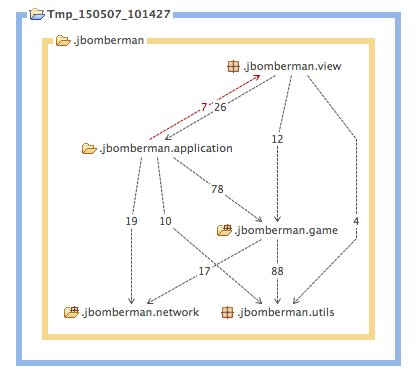
\includegraphics[width=0.85\textwidth]{stan}
\end{center}
\begin{center}
  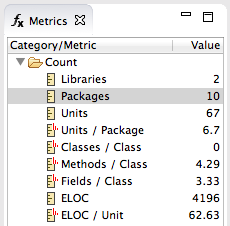
\includegraphics[width=0.85\textwidth]{stan-metrics}
\end{center}
\subsection{Beschreibung}
Zwar konnten einige Abhängigkeiten gelöst werden (zwischen utils und Game) -> 
jedoch konnte aus Zeitgründen und nicht sofortiges funktionieren die 
Abhängigkeit zwischen Application und View nicht gelöst werden.
\newpage
\section{Findbugs}
Findbugs wurde zur statischen Code Analyse verwendet, um Fehler im Code 
aufzuzeigen.
\begin{center}
 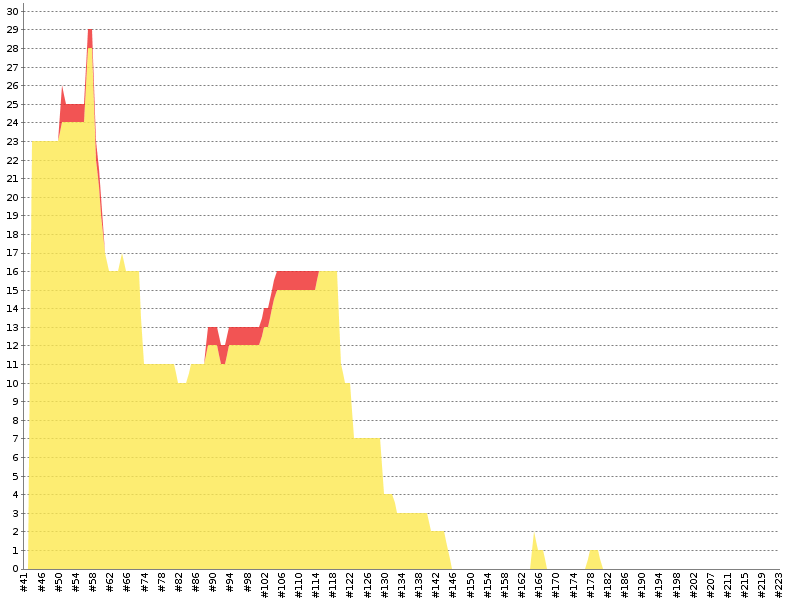
\includegraphics[width=0.85\textwidth]{findbugs}
\end{center}
\subsection{Beschreibung}
Am Anfang des Projekt waren noch einige Warnungen vorhanden, 
diese wurden jedoch dann nach und nach beseitigt.
Zum Schluss bestehen also keine Findbugs Warnungen mehr.
\newpage
\section{Jacoco}
Jacoco wurde zur Analyse der Test Code Coverage gebraucht (als Ant Task).
\subsection{Beschreibung}
Jedoch wurde zu keinem Zeitpunkt eine genügend hohe Test Code Coverage 
erreicht was das einfügen des Graphen unnötig macht -> siehe 
\href{http://se2p.zonk.io/jenkins/}{Jenkins}.
\newpage
\section{Eclipse Metrics}
Eclipse Metrics wurde für die Statistik des Projekts zum Abschluss eingesetzt.
\begin{center}
 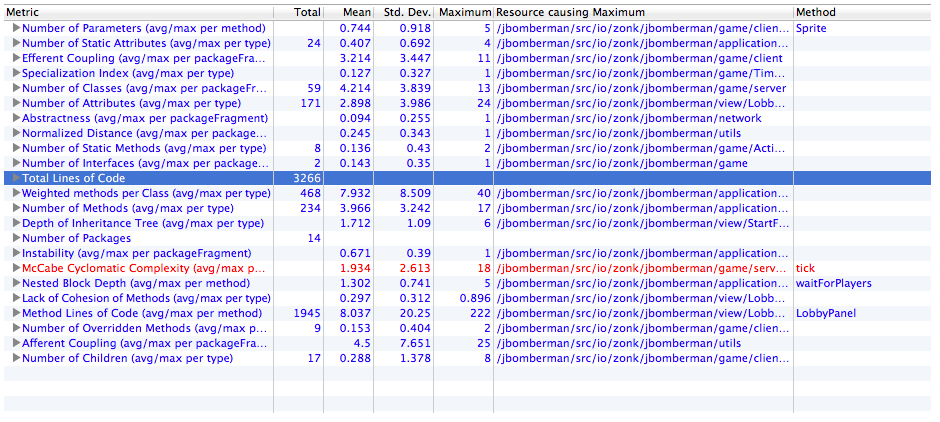
\includegraphics[width=0.85\textwidth]{metrics}
\end{center}
\subsection{Beschreibung}
Dabei kommen wir auf eine Total Lines of Code von 3266.
\end{document}